\documentclass[12pt]{article}

\usepackage{lineno}

\usepackage{rotating}
\usepackage{tikz}
\usepackage[round]{natbib}
\usepackage{crop}
\usepackage{graphicx}
\usepackage{amsmath}
\usepackage{array}
\usepackage{color}
\usepackage{amssymb}
\usepackage{flushend}
\usepackage{stfloats}
\usepackage{amsthm}
\usepackage{times}
\usepackage{tabularx}
\usepackage{pstricks}
\usepackage{hyperref}
\usepackage[left=0.75in,
 right=0.75in,
 top=1.25in,
 bottom=1.25in]{geometry}
 
\def\bibliofont{22pt}


\newcommand{\ednote}[1]{{\color{red}[[XXX #1 ]]}} 
 
 
\begin{document}

\title{Blind dating: A phylogenetic approach to dating HIV reservoir sequences}

\author{Joshua Horacsek$^{1,2}$, Jeffrey B. Joy$^2$, \\ Zabrina L. Brumme$^{1,2}$, and Art F.Y. Poon$^{1,2,3}$}
% 1 Simon Fraser University
% 2 BC Centre for Excellence in HIV/AIDS
% 3 University of British Columbia
\baselineskip 22pt
\pagewiselinenumbers

\date{}
\maketitle
%\begin{abstract}

Background: The ability of HIV to persist within latent cellular reservoirs represents a major barrier to cure. The timing of establishment of individual viral reservoirs over the infection course could influence their susceptibility to elimination by immune-mediated or therapeutic approaches. However, “dating” methods to accurately estimate the age of reservoir sequences remain scarce. We propose a simple method to date suspected reservoir sequences using phylogenetic approaches. 

Method: Simulated sequence data for model validation were generated using INDELible version 1.03.  Published longitudinal clonal sequences from untreated HIV-infected individuals with estimated dates of infection were obtained from the Los Alamos National Laboratory database. Maximum-likelihood phylogenies were reconstructed with PhyML. Phylogenies were rooted by determining the location of the root that minimized the root-mean-square error between root-to-tip distances and known dates of sampling. The root-to-tip distances of latent sequences were mapped to the optimal regression line to estimate their establishment date, which was assumed to precede their sample dates by an unknown amount.
 
Results: We validated the root-to-tip method using simulated data and published longitudinal clonal sequence datasets from untreated HIV-1 infected individuals with known infection dates. For each dataset, arbitrary selections of up to 10% of sequences were handled as latent by censoring their respective sample dates.  The method accurately recovered these missing sample dates when the phylogeny conformed to a strict molecular clock, as was the case for simulated data (SOME KIND OF PERFORMANCE METRIC HERE?  MEAN RMSE?). A strict clock model could not be rejected in the majority of empirical within-host data sets. When applied to HIV DNA sequences in phylogenies containing dated HIV RNA sequences, we observed that the predicted dates tended to precede dates of sampling, which was consistent with latency (MAYBE SOME METRIC HERE LIKE MEAN DISCORDANCE).

Conclusions:
Given a known phylogeny comprised of longitudinal plasma HIV-1 RNA sequences, the establishment dates of “unknown” (reservoir) sequences can be reliably estimated when within-host HIV sequence evolution conforms to a molecular clock. Future studies will test this method on empirically derived longitudinal within-host HIV deep sequence data and extend the method to work under alternative clock models.

Keywords: 
HIV, Latency, Cellular Reservoirs, Phylogenetics, Linear Regression

%\end{abstract}

\section * {Introduction} \label{sec:intro}

Latent viral reservoirs within HIV-1 infected individuals are a major obstacle on the path to developing HIV cure strategies \citep{Pace11}. 
Reservoirs are cells that contain integrated viral DNA and have entered a dormant state in which they not only have a lowered rate of virion production, but may also persist within an individual for several years or more.
Even though highly active antiretroviral therapy (HAART) can reduce a patient's viral load to below detectable levels, latent reservoirs will eventually reseed an infection if a patient halts treatment \citep{Joos08, Pomerantz03, Richman09}.


Due to selective pressure from the host's immune system and the high mutation rate and short generation time of the virus, HIV-1 evolves very quickly throughout the course of infection \citep{Alizon13, Shankarappa99, Rambaut04}. 
Consequently, it is feasible to reconstruct a phylogeny that models the pattern of common ancestry from the genetic differences among virus lineages that have been sampled from a given infection. 
%Additionally, to some degree, one can trust the sampling time for active sequences to be in accordance with the actual age of the sequence.
The phylogeny can be subsequently rescaled to chronological time by fixing the tips to their respective dates of sample collection, and using this additional information to directly estimate the rate of evolution under a molecular clock model \citep{Rodrigo99}.
For sequences originating from the active population of virus, it is not unreasonable to assume that the rate of molecular evolution is relatively constant -- in other words, that it adheres to a `molecular clock' model \citep{Leitner99, Kuhner95, Korber00}. 
%However for suspected latent sequences, the sampling time may not be in accordance with the expected age of the sample -- yet, if the molecular clock holds true, one can use the expected amount of evolution from the phylogenetic reconstruction to reconstruct the expected age of a sample.
Once the virus has integrated itself into a cell, however, the rate at which it accumulates mutations becomes negligible compared to the rate at which the active population in plasma evolves. 
Thus, integration transiently halts the evolution of that particular virus lineage. 
%If one looks at the phylogeny of the samples from an infected patient, and the branch lengths this phylogeny represent time, then 
Viral latency can be manifested by a discordance between a sample's actual collection time and its apparent age based on its sequence divergence from other lineages (Figure \ref{fig:latenttree}). 
Therefore, it may be possible to use a molecular clock model to reconstruct the dates that a given virus lineage became latent.

Not much is known about when latent reservoirs are established over the course of an infection. 
The chronology of their establishment is of interest as the distribution of ages of the stored virus(es) may provide information concerning the types of adaptations that the virus may have accumulated. 
Specifically, it may have an influence on how those infected cells react to immune-mediated and/or therapeutic treatments. 
Previous studies have looked at the population dynamics of different classes of the virus within host, modeled those classes with systems of ordinary differential equations, then fit those models to empirical data \citep{Althaus14}. 
There has also been work that attempts to characterize latent sequences using a relaxed clock approach \citep{Immonen14}. 
However, there has not been much work towards assigning dates to HIV sequences that are suspected to be latent, or qualitatively assessing the distribution of collection-age differences for suspected latent samples.

We propose a simple framework to estimate dates of latent reservoirs that utilizes the assumption of a strict molecular clock -- that the expected number of substitutions per site is linearly related to time \citep{Ho14} --  on the evolution of HIV within host. 
Our method extracts timing information from the phylogenetic relationship between the virus sampled at various time-points along the infection. 
We first construct a phylogeny containing both cellular HIV DNA and plasma HIV RNA derived sequences from the same patient, then parameterize a strict clock model on that tree based solely on the collection dates of the HIV RNA sequences. 
Since the root of this phylogeny is typically unknown, we employ either root-to-tip regression \citep{Korber00} or outgroup rooting to estimate the location of the root in the tree. 
We assume that sequences derived from cellular HIV DNA such as that extracted from peripheral blood mononuclear cells (PBMCs) are potentially derived from latent reservoirs, and have therefore have effectively stopped evolving.
Although sequences derived from plasma HIV RNA may potentially be descended from reactivated latent virus lineages, we assume that this affects only a minority of sequences derived from blood plasma on the time scales represented by the longitudinal data sets in our study (see below).

To assess the sensitivity of our method, we first simulated sequence data with no viral latency and evaluated the accuracy of predicting sample collection times from a strict molecular clock model that was fit to a training subset of the sequences. 
%We then simulated and evaluated sequences from a model that exhibits simplified latent behavior. 
Next, we evaluated the same model on sequence data that was simulated under a model that included viral latency in the form of a variable molecular clock.
To mimic the types of results we expected from our first test, we used a collection of published longitudinal patient-derived sequence data sets comprising exclusively plasma-derived HIV sequences \citep{McCloskey14} to evaluate the accuracy of date reconstruction for sequences with censored dates. 
Finally, we tested our methodology on another collection of longitudinal patient-derived data sets comprising both PBMC and plasma sequences. 
If the molecular clock assumption holds for all sequences, and latency merely implies a ``pause'' in the evolution of a sequence, then the clock should be a reliable source of information for dating latent sequences.

\begin{figure} \label{fig:latenttree}
	\centering
	\scalebox{5}{%LaTeX with PSTricks extensions
%%Creator: inkscape 0.91
%%Please note this file requires PSTricks extensions
\psset{xunit=.5pt,yunit=.5pt,runit=.5pt}
\begin{pspicture}(85,53)
{
\newrgbcolor{curcolor}{0 0 0}
\pscustom[linewidth=0.38699999,linecolor=curcolor]
{
\newpath
\moveto(77.921134,4.13898)
\lineto(5.1912118,4.13898)
\lineto(5.1912118,20.207747)
}
}
{
\newrgbcolor{curcolor}{0 0 0}
\pscustom[linewidth=0.38699999,linecolor=curcolor]
{
\newpath
\moveto(65.799478,25.564002)
\lineto(29.434525,25.564002)
\lineto(29.434525,36.276514)
}
}
{
\newrgbcolor{curcolor}{0 0 0}
\pscustom[linewidth=0.38699999,linecolor=curcolor]
{
\newpath
\moveto(41.556173,46.989025)
\lineto(29.434525,46.989025)
\lineto(29.434525,36.276514)
}
}
{
\newrgbcolor{curcolor}{0 0 0}
\pscustom[linewidth=0.38699999,linecolor=curcolor]
{
\newpath
\moveto(29.434525,36.276514)
\lineto(5.1912118,36.276514)
\lineto(5.1912118,20.207747)
}
}
{
\newrgbcolor{curcolor}{0 0 0}
\pscustom[linewidth=0.38699999,linecolor=curcolor]
{
\newpath
\moveto(4.4639148,20.207747)
\lineto(5.1912118,20.207747)
}
}
{
\newrgbcolor{curcolor}{0 0 0}
\pscustom[linestyle=none,fillstyle=solid,fillcolor=curcolor]
{
\newpath
\moveto(81.87934379,5.47198716)
\lineto(81.87934379,5.02049697)
\curveto(81.73520608,5.15474288)(81.58117656,5.25507403)(81.41725524,5.32149043)
\curveto(81.25474704,5.38790683)(81.08164047,5.42111503)(80.89793554,5.42111503)
\curveto(80.53617814,5.42111503)(80.25920764,5.31018551)(80.06702402,5.08832648)
\curveto(79.8748404,4.86788057)(79.77874859,4.54851662)(79.77874859,4.13023462)
\curveto(79.77874859,3.71336575)(79.8748404,3.3940018)(80.06702402,3.17214277)
\curveto(80.25920764,2.95169685)(80.53617814,2.84147389)(80.89793554,2.84147389)
\curveto(81.08164047,2.84147389)(81.25474704,2.87468209)(81.41725524,2.94109849)
\curveto(81.58117656,3.00751489)(81.73520608,3.10784604)(81.87934379,3.24209195)
\lineto(81.87934379,2.79484111)
\curveto(81.72955362,2.69309684)(81.5705782,2.61678864)(81.40241754,2.5659165)
\curveto(81.23566999,2.51504437)(81.05903063,2.4896083)(80.87249947,2.4896083)
\curveto(80.39345355,2.4896083)(80.01615188,2.63586569)(79.74059449,2.92838046)
\curveto(79.4650371,3.22230834)(79.3272584,3.6229264)(79.3272584,4.13023462)
\curveto(79.3272584,4.63895596)(79.4650371,5.03957402)(79.74059449,5.33208879)
\curveto(80.01615188,5.62601668)(80.39345355,5.77298062)(80.87249947,5.77298062)
\curveto(81.06185686,5.77298062)(81.23990933,5.74754455)(81.40665688,5.69667242)
\curveto(81.57481755,5.6472134)(81.73237985,5.57231831)(81.87934379,5.47198716)
\closepath
}
}
{
\newrgbcolor{curcolor}{0 0 0}
\pscustom[linestyle=none,fillstyle=solid,fillcolor=curcolor]
{
\newpath
\moveto(67.94040944,25.49054575)
\lineto(67.94040944,24.41103725)
\lineto(68.57982581,24.41103725)
\curveto(68.79428027,24.41103725)(68.95281869,24.45511225)(69.05544107,24.54326224)
\curveto(69.15937912,24.63272791)(69.21134815,24.76889991)(69.21134815,24.95177825)
\curveto(69.21134815,25.13597227)(69.15937912,25.27148644)(69.05544107,25.35832076)
\curveto(68.95281869,25.44647075)(68.79428027,25.49054575)(68.57982581,25.49054575)
\lineto(67.94040944,25.49054575)
\closepath
\moveto(67.94040944,26.70227923)
\lineto(67.94040944,25.81420095)
\lineto(68.53048813,25.81420095)
\curveto(68.72520752,25.81420095)(68.86993138,25.85038191)(68.96465973,25.92274385)
\curveto(69.06070376,25.99642145)(69.10872577,26.10825353)(69.10872577,26.25824009)
\curveto(69.10872577,26.40691097)(69.06070376,26.51808522)(68.96465973,26.59176282)
\curveto(68.86993138,26.66544043)(68.72520752,26.70227923)(68.53048813,26.70227923)
\lineto(67.94040944,26.70227923)
\closepath
\moveto(67.54176097,27.02988145)
\lineto(68.56009074,27.02988145)
\curveto(68.86401086,27.02988145)(69.0982004,26.96672921)(69.26265934,26.84042474)
\curveto(69.42711828,26.71412028)(69.50934775,26.53453111)(69.50934775,26.30165725)
\curveto(69.50934775,26.12141025)(69.46724626,25.97800205)(69.38304328,25.87143266)
\curveto(69.29884031,25.76486326)(69.17516718,25.69842185)(69.01202391,25.67210842)
\curveto(69.20805897,25.63000693)(69.36001903,25.54185694)(69.4679041,25.40765844)
\curveto(69.57710484,25.27477562)(69.6317052,25.10834317)(69.6317052,24.90836109)
\curveto(69.6317052,24.64522679)(69.54223954,24.44195553)(69.36330821,24.29854734)
\curveto(69.18437688,24.15513914)(68.92979444,24.08343504)(68.59956088,24.08343504)
\lineto(67.54176097,24.08343504)
\lineto(67.54176097,27.02988145)
\closepath
}
}
{
\newrgbcolor{curcolor}{0 0 0}
\pscustom[linestyle=none,fillstyle=solid,fillcolor=curcolor]
{
\newpath
\moveto(68.8325765,47.98448198)
\lineto(68.33071752,46.62360158)
\lineto(69.33626709,46.62360158)
\lineto(68.8325765,47.98448198)
\closepath
\moveto(68.62377386,48.34897081)
\lineto(69.04321075,48.34897081)
\lineto(70.08539237,45.6143888)
\lineto(69.70075592,45.6143888)
\lineto(69.45165803,46.31589242)
\lineto(68.21898978,46.31589242)
\lineto(67.96989189,45.6143888)
\lineto(67.57976063,45.6143888)
\lineto(68.62377386,48.34897081)
\closepath
}
}
{
\newrgbcolor{curcolor}{0 0 0}
\pscustom[linewidth=0.39463133,linecolor=curcolor,linestyle=dashed,dash=0.7892628 0.7892628]
{
\newpath
\moveto(41.217255,46.97727)
\lineto(65.885506,46.9308)
}
}
\rput(42,52){\psscalebox{0.3}{$t$}}
\rput(66,52){\psscalebox{0.3}{$t^\prime$}}
\end{pspicture}
}
	\caption[Example of latent behavior]{The dotted line in the above figure is an example of latency. 
	Sequence A was archived at time $t$, and was collected at the same time as sequence B, at time $t^\prime$ -- a drift of $t^\prime - t$ is expected. 
	If the molecular clock assumption holds true, the MRCA is known, and B and C are reliable time-points, then the date at $t$ can be inferred from from the expected amount of evolution for B from the root.}
\end{figure}

\section{Methods} \label{sec:methods}
\subsection{Simulated Data} \label{subsec:simdata}
We first used seed phylogenies generated via a birth death model (with birth and death rate equal to $5\times 10^{-3}$ and with a 5\% chance of being sampled) in the R package TreeSim \citep{TreeSim, Stradler13, Boskova14}, and assign a clock to these trees (with rate$=3\times 10^{-3}$ substitutions per site/day, and with noise pulled from a normal distribution with $\sigma=5\times 10^{-5}$.
We then used INDELible 1.03 \citep{Indelible09} to simulated nucleotide sequences along these seed phylogenies with an HKY85 \citep{HKY85} substitution model, and  parameters set from a maximum likelihood estimate of published within host data \citep{McCloskey14}. 
From these simulated sequences a maximum likelihood phylogeny was then reconstructed with RAxML \citep{Raxml14}. In total, we generated 50 trees without latency, each having 100 tips. 

To generate the trees that had observable latency, we took a similar approach to that of \cite{Immonen14}. 
We randomly selected a branch within a seed phylogeny then scaled it by a random value between $0.1$ and $0.9$, to assure that the phylogeny had sufficiently many latent tips, we rejected all such trees that had less than 40 and more than 60 latent tips. 
We then recorded both the simulated age and simulated collection time, then generated sequences along these latent seed trees with INDELible 1.03 \citep{Indelible09} and the same parameters above. 
From these simulated sequences a maximum likelihood phylogeny was then reconstructed with RAxML \citep{Raxml14}.
For these data, we generated an additional 50 trees with 100 tips, bringing the total amount of simulated data to 100 trees with 100 tips each. 


\subsection{Data Collection} \label{subsec:dcollection}
We collected two distinct sets of data for our experiments, the first is the {\em plasma} data-set, which contains data collected from studies in which only viral RNA had been collected. 
The second data-set, the {\em mixed} data-set, contained sequences from studies in which both viral RNA in plasma and integrated viral DNA from PBMC cells had been collected.

Specifically, the {\em plasma} data-set \citep{McCloskey14} is a previously assembled and cleaned data-set from the Los Alamos HIV Database (\href{http://www.hiv.lanl.gov/}{http://www.hiv.lanl.gov/}). 
This data set contains 335 data sets from 232 patients, with a total of over 19,000 sequences \citep{McCloskey14} containing mostly longitudinal samples collected from plasma. 
From this set we selected treatment naive patients with two or more clonal or single-genome sequences available at each time point, with a known time-line relative to one of several reference points: HIV infection, seroconversion or presentation of symptomatic seroconversion illness. 
The samples were collected within 6 months (186 days) of this reference point, and at least one of the subsequent (“follow-up”) time points occurred a minimum of 6 months after baseline.
Patients who had been classified as ``superinfected'' were also excluded, and the samples were taken from the {\em env} region of the HIV-1 genome \citep{McCloskey14}. 
From this data-set we use \anote{X} plasma samples from \anote{Y} specific patients. 


For the {\em mixed} data-set, we used the Los Almos advanced search interface (\href{http://www.hiv.lanl.gov/}{http://www.hiv.lanl.gov/}) to identify subjects who have had both viral RNA and integrated DNA from PBMC cells collected over various time points -- we selected individuals from published studies that had well-characterized partial {\em env}. 
There was no condition for the time between sample collections. 
\anote{X} individuals were included with plasma samples from at least 2 time points (table \ref{tab:patients}).
A total of \anote{X} partial {\em env} sequences from blood plasma, and \anote{Y} partial {\em env} sequences from PBMC cells were used in our analysis. 
We utilized samples from treatment naive individuals \citep{Shankarappa99, Novitsky09}, from individuals that had been treated via HAART \citep{Llewellyn06}, and individuals that had been on HAART, but ceased treatment \citep{Fischer04}. 
 
\begin{table*}[!ht]
\def\arraystretch{1.3}%
\begin{center}
\begin{tabular}{llrrrrrr} 

Reference & Patient ID & \multicolumn{3}{c}{Sequences} & \multicolumn{3}{c}{Time points}\\ 
 &  & Plasma & PBMC & Total & Plasma & PBMC & Total\\
\hline
\cite{Shankarappa99} & 820 &       50 &       87 &      137 &        5 &       10 &       15  \\
& 821 &      76 &      192 &      268 &        7 &       17 &       17   \\ 
& 822 &      32 &       98 &      130 &        3 &       10 &       10   \\ 
& 824 &     100 &      107 &      207 &        7 &        9 &       13   \\ 
& 10137 &     24 &      106 &      130 &        2 &       10 &       12  \\ 
& 10138 &     82 &      119 &      201 &        6 &       13 &       16  \\
& 10586 &     16 &      121 &      137 &        2 &       12 &       14  \\ 
& 13889 &    151 &      132 &      283 &       13 &       14 &       18  \\ 
 \cite{Fischer04} & 10769 &    229 &       96 &      325 &       10 &        4 &       11  \\ 
& 10770 &    190 &       31 &      221 &       11 &        2 &       11  \\ 
\cite{Llewellyn06} & 16616 &     16 &       95 &      111 &        2 &        5 &        5  \\ 
& 16617 &     16 &       89 &      105 &        2 &        5 &        5  \\ 
& 16618 &     25 &       75 &      100 &        2 &        5 &        6  \\ 
& 16619 &     13 &       60 &       73 &        2 &        6 &        6  \\ 
\cite{Novitsky09} & 34382 &     37 &        5 &       42 &        3 &        1 &        4  \\ 
& 34391 &     13 &       38 &       51 &        3 &        5 &        6  \\ 
& 34393 &     25 &       74 &       99 &        2 &        6 &        7  \\ 
& 34396 &      23 &       46 &       69 &        2 &        5 &        5 \\ 
& 34397 &      26 &       25 &       51 &        2 &        2 &        4  \\ 
& 34399 &      61 &       88 &      149 &        5 &        9 &       12  \\ 
& 34400 &      54 &       23 &       77 &        4 &        1 &        5  \\ 
& 34405 &      27 &       29 &       56 &        3 &        2 &        4  \\ 
& 34408 &       5 &       73 &       78 &        2 &        8 &        8 \\ 
& 34410 &      35 &       60 &       95 &        2 &        6 &        6 \\ 
& 34411 &      25 &       43 &       68 &        3 &        3 &        6   \\ \hline
\end{tabular}
\end{center}
  \caption{Summary of all the patient data collected from the HIV LANL database -- Patient ID corresponds to the Los Alamos database's Patient ID \citep{LosAlamos}.
   }\label{tab:patients} 
\end{table*}

\subsection{Sequence Aligment} \label{subsec:seqalign}
When applicable, we used the built in MUSCLE 3.8.31 \citep{Muscle04} interface within AliView \citep{AliView14} to align the sequences, which were then visually inspected and cleaned. 
Alignments were trimmed to the interval in which at least  50\% of sequences within the data set had sequence coverage over each codon.
Our simulated sequences contained no insertions or deletions, so no alignment was necessary. 
Additionally, the plasma data-set \citep{McCloskey14} had already been aligned and cleaned, so no further alignment was performed.


\subsection{Phylogenetic Reconstruction} \label{subsec:phylo}
In all experiments, our reconstructed phylogenies were maximum likelihood phylogenies reconstructed in RAxML \citep{Raxml14} using the GTR+$\Gamma$ model.
We did not attempt to use BEAST \citep{BEAST} to reconstruct any phylogenies from our data.
Leaving dates unspecified on the number of tips would have drastically increased the dimensionality of the problem, and we would therefore need a prohibitively large amount of samples from the MCMC chain to assure convergence to the posterior distribution.


To root these trees, either outgroup rooting against the HIV-1 B ancestor reconstruction, or a modified version of RTT regression \citep{APE}. 
Classically, RTT regression considers all tips and chooses the root that minimizes some error metric between the maximum likelihood estimated clock and the tip dates. 
For this application, we simply ignore the tips that are undetermined (either censored or otherwise unknown) in the optimization of the root. 
Our synthetic data was only rooted using this modified RTT scheme, for all real data, both outgroup rooting and root-to-tip regression were used to root the phylogeny. 


\subsection{Date Reconstruction} \label{subsec:daterecon}
Once the trees had been rooted, to reconstruct dates, a general linear model with the normal family was constructed. 
The expected amount of evolution was taken to be the response and the sampling dates of the data were taken as the input. 
These models were only trained over the uncensored/plasma data for the simulated and real data sets respectively.

\subsection{Hypothesis Testing} \label{subsec:hypot}
To screen for data are amenable to our analysis, we used the nested log ratio test \citep{Ho14}. 
Our null model was a linear model with zero slope over the expected amount of evolution over time. 
We rejected any sequence data-sets whose phylogeny couldn't reject the null model with threshold $\alpha=0.01$.


\subsection{Experiments} \label{subsec:experiments}
Our first validation experiment on synthetic data was preformed as such: First we choose 50\% of the tips of a phylogeny and censored those dates, we next used root-to-tip regression \citep{APE} on the remaining data to calibrate the molecular clock for the tree. Finally, for each censored date, we reconstructed the expected date using the expected number of substitutions.

In all of our experiments, before any analysis is done, all times are re-scaled to lie between $0$ and $1$. This is calculated as $$ \text{new time} = \frac{\text{time} - \text{min time}}{\text{max time} - \text{min time}}$$ this gives normalized time. Errors are then calculated from this number, which we call normalized error. On the left figure \ref{fig:results1} shows a linear regression over either simulation time or time from a reference point (for patient data). On the right side of figure \ref{fig:results1}, is the superposition of an error density estimate for each data set within a category. 

\section{Results} \label{sec:results}
%On the left figure \ref{fig:results1} shows a linear regression over either simulation time or time from a reference point (for patient data). On the right side of figure \ref{fig:results1}, is the superposition of an error density estimate for each data set within a category. 

\begin{sidewaysfigure} \label{fig:results1}
	\centering
	\includegraphics[trim=0cm 0cm 0cm 6cm, clip=true, scale=0.425]{figures/simulated.pdf} \\
	\includegraphics[trim=0cm 0cm 0cm 7cm, clip=true,scale=0.425]{figures/simulated_latent.pdf}\\
	\caption[Examples]{\anote{Add legend, change points, change shading, explain point colouring, explain mean and median lines.}}
\end{sidewaysfigure}

\begin{sidewaysfigure} \label{fig:res}
	\centering
	\includegraphics[trim=0cm 0cm 0cm 7cm, clip=true,scale=0.425]{figures/ancre.pdf}\\
	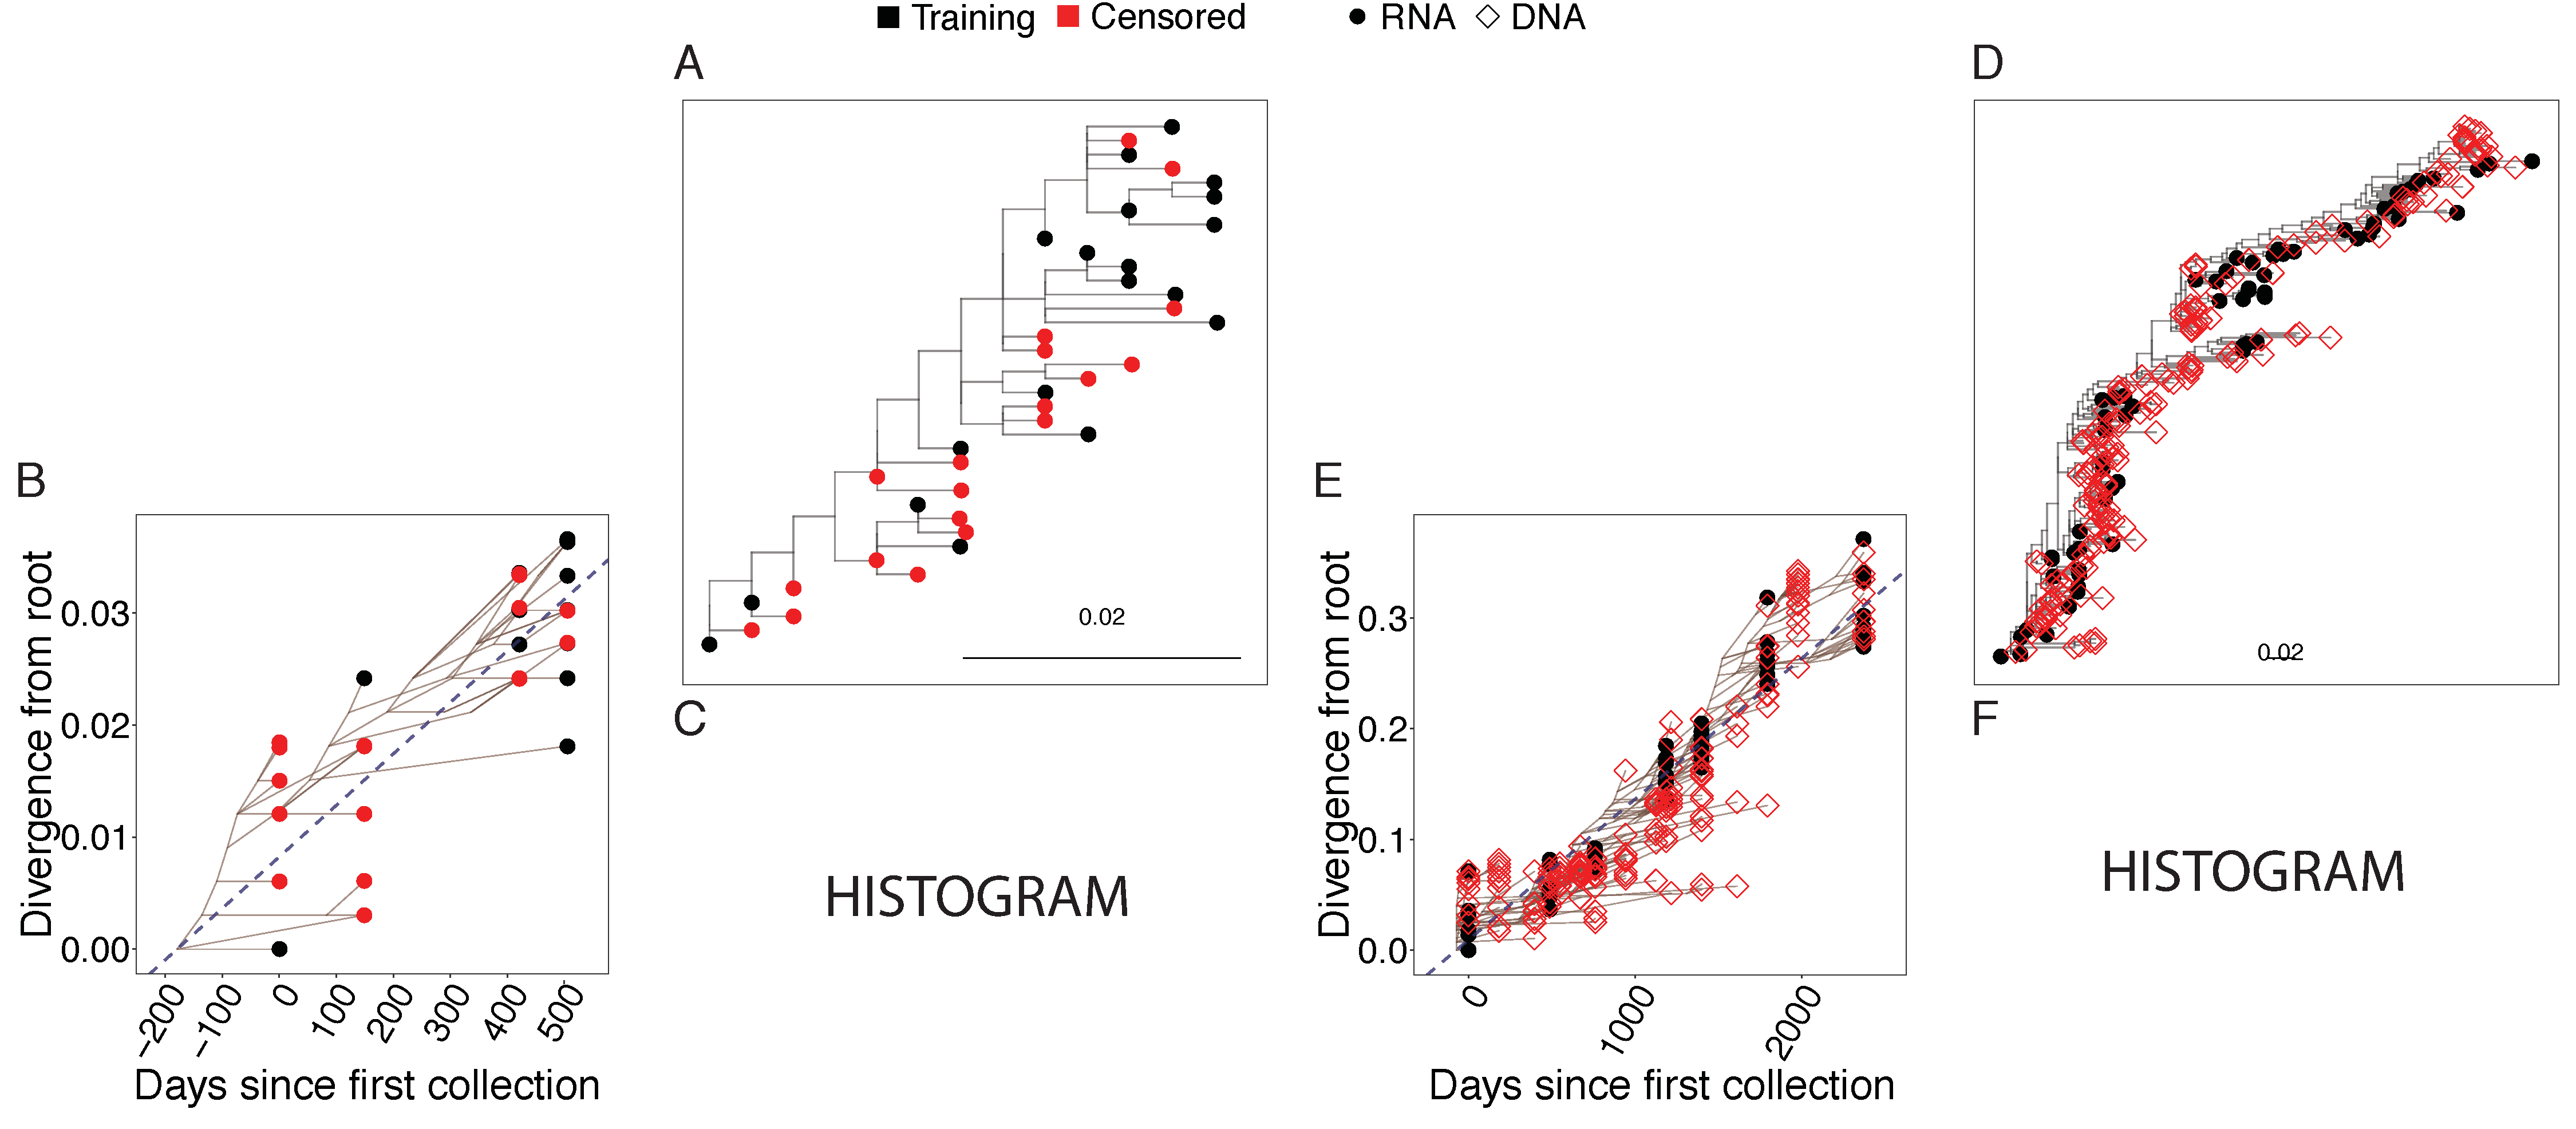
\includegraphics[trim=0cm 4cm 0cm 7cm, clip=true,scale=0.425]{figures/lanl.pdf}
	\caption[Examples]{\anote{Add legend, change points, change shading, explain point colouring, explain mean and median lines.}}
\end{sidewaysfigure}


\subsection{Simulated Data} \label{sec:sim_results}
Figure \ref{fig:results1} A shows that the clock is a reliable source of information in this case. Quantitatively, the censored data points are close to the regression line, and the difference density is heavily peaked around 0. Averaged over all simulated data sets, the average mean square error was \anote{X}, and the average median and mean difference were \anote{Y} and \anote{Z} respectively.

Figure \ref{fig:results1} B shows the regression over the calibration dates and the simulated collection dates. Note that these dates are not the actual. In this experiment, the density plot is shifted to the right, exemplifying latent behavior. Averaged over all simulated data sets, the average mean square error was \anote{X}, and the average median and mean difference were \anote{Y} and \anote{Z} respectively. However, when we utilized the known sample ages (as opposed to the collection dates) then measured the same metrics, averaged over all simulated data sets, the average mean square error was \anote{X}, and the average median and mean difference were \anote{Y} and \anote{Z} respectively.

\subsection{Plasma data-set} \label{sec:rna_only}

Figure \ref{fig:results1} C shows the regression over the calibration dates and the collection date. Averaged over all simulated data sets, the average mean square error was \anote{X}, and the average median and mean difference were \anote{Y} and \anote{Z} respectively. The superposition of the difference density plots shows similar behavior to that of \ref{sec:sim_results}, except with a wider distribution, and more variation. Since there is inherently more noise in this data, this is expected. 

\subsection{Mixed data-set} \label{sec:mixed_data}

Figure \ref{fig:results1} D shows the regression over the calibration dates and the simulated collection date. In this case, we do not know the actual date of archival.  The superposition of the difference density plots shows similar behavior to that of the latent simulated data, except \anote{need new plots for this}.  

The patients that had received treatment at some point generally failed the hypothesis testing -- there was only one patient that did not. This suggests that after a patient begins treatment, the assumption of a molecular clock over their phylogeny is too strong. 

\section{Discussion} \label{sec:discuss}
The simulated data are unsurprising, the RNA data too. Patient data trends and analysis.
\section{Conclusion} \label{sec:conclusion}
Once the trees had been rooted, a general linear model with the normal family was constructed with the with expected number of substitutions as the input, and sampling time as the response. For all experiments using patient data, this fit was only over the plasma data, and the PBMCs expected subs were used as input. From this, we collected the difference between the observed sampling date, and the predicted date. 
Once the trees had been rooted, a general linear model with the normal family was constructed with the with expected number of substitutions as the input, and sampling time as the response. For all experiments using patient data, this fit was only over the plasma data, and the PBMCs expected subs were used as input. From this, we collected the difference between the observed sampling date, and the predicted date. 
Talk about what we saw.
Talk about what can still be done.


%\section{Acknowledgments} \label{sec:ackn}
%The authors would like to thank --.

\bibliographystyle{natbib}
%\bibliographystyle{achemnat}
%\bibliographystyle{plainnat}
%\bibliographystyle{abbrv}
%\bibliographystyle{bioinformatics}
%\bibliographystyle{plain}

\bibliography{main}

\end{document}
